\chapter{Coded target}
\label{Chap:CodedTarget}

%-----------------------------------------------------------------------
%-----------------------------------------------------------------------
%-----------------------------------------------------------------------

\section{Todo}

\begin{itemize}
      \item  {\tt 2023-12-14-CurTestClino/Calib-1/Processing/}  target partially occluded are recognized as others,
	      for example {\tt 043\_0078.JPG}, target {\tt 66 (?)} is interpreted as {\tt 34} ;
\end{itemize}


%-----------------------------------------------------------------------
%-----------------------------------------------------------------------
%-----------------------------------------------------------------------

\section{Introduction}

%-----------------------------------------------------------------------

\subsection{Generality}

Coded target are usefull in photogrammetry for different purpose : 
fully automated pipelin even with low texture scenes, high accuracy metrologic application.
The service offered by MMVII regarding coded target are :

\begin{itemize}
    \item generate a bit encoding (set of vector of bit) taking into account 
           user's requirement;

    \item generate a geometry specification taking into account
           user's requirement;

    \item generate printable images of all, or a subset, of coded target system;

    \item generate simulation images where coded target are included;

    \item detect the coded target;

    \item validate uncoded target in a second iteration  (once we know their approximate location).

\end{itemize}


%-----------------------------------------------------------------------

\subsection{Criterion for a coded target system}

There are many criteria for selecting a coded target system, among which we can cite :

\begin{itemize}
    \item number of possible different codes we need;

    \item robustness of detection, false positive and true negative,  depending on
	    different condition  (noise, ligthing , occlusion,  deformation, blurring \dots);

    \item threshold of detectability : what minimal size (in pixel) must have target in images
	    for detecting them;

    \item potentiel speedness of detection ;

    \item potential accuracy of automatic measurement in images;

    \item accuracy and easyness of measurement by topography on the field.

\end{itemize}


%-----------------------------------------------------------------------

\subsection{Main variants}

There is obviously no system optimal for all theses criteria, and the choice will have to
be fine-tuned according to specific application.
For now {\tt MMVII} offer $4$ main variant of coded target . As we will see, these $3$ systems are in
fact the specific parametrization of the same global system.

\begin{figure}
\centering
   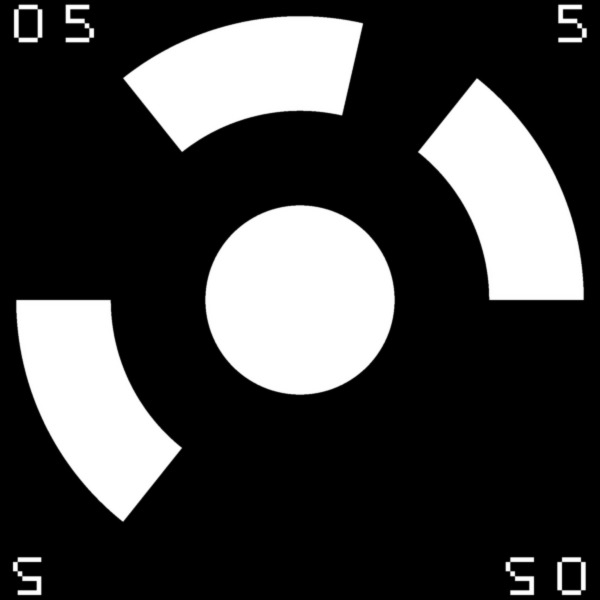
\includegraphics[width=4cm]{Methods/Images/CERN-055.jpg}
   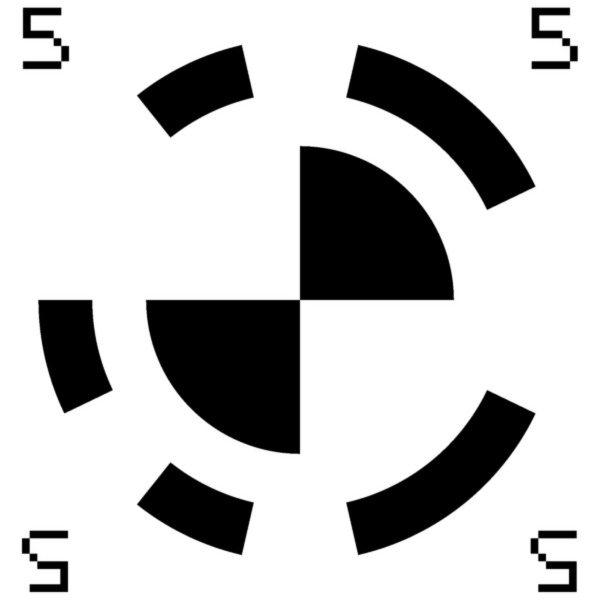
\includegraphics[width=4cm]{Methods/Images/IgnIndoor-55.jpg}
   
\includegraphics[width=4cm]{Methods/Images/IGNDRonSym_55.jpg}
   
\includegraphics[width=4cm]{Methods/Images/IGNDroneTop_55.jpg}
    \caption{Target (1) {\bf CERN} Compatible with commercial software 
                    (2) {\bf IgnIndoor} Checkboard circular target 
		    (3) {\bf IGNDroneTop} and (4) {\bf IGNDroneSym} Checkboard linear target
            }
\label{fig:CodedTarget}
\end{figure}

  %  -  -  -  -  -  -  -  -  -  -  -  -  -  -  -  -  -  -  -  -  -  -  -  -  -  -  -  -  -  -  -  -
\subsubsection{Circular target variant}

In these variant the centre target is simply a circle.  


These kind of target have been added in {\tt MMVII} as they are very common in commercial
software (AICON-3D , photomodeler, Agisoft). The variant will be named {\bf CERN}, refering to
its first usage in {\tt MMVII}.


%-----------------------------------------------------------------------
\subsubsection{Checkboard coded target}

In the other variants, the central target is a checkboard because it's  easier to input the center
by topography: 


\begin{itemize}
     \item  The first variant the code is circular, it will be named {\bf IGNIndoor},
	     it is adapted for indoor topgraphy

     \item  In the third and four variant the code is linear, they correspond to the following
	     practicle constraint coming from drone survey: we want to print the targt with a standard printer
            (size  {\tt A4} or {\tt  A3}),  and want to maximize the size of check board because
            we need that the in the image, there is sufficient pixel for detection, and with drone the
		resolution can be typically $1cm$ to $2cm$ (at $2cm$  a {\tt A3} has $15$ pixel width).
\end{itemize}

%-----------------------------------------------------------------------
%-----------------------------------------------------------------------
%-----------------------------------------------------------------------

\section{Encoding and decoding conception}


%-----------------------------------------------------------------------

\subsection{General principal}

The coding conception of such systems is made while thinking
about the decoding part  that will have to be (if possible) : non ambiguous,
robust, fast \dots   Generally (and always in {\tt MMVII})  target are made of two parts :

\begin{itemize}
    \item a fix part, like the circle or the checkboard,  as this part is fixed
         its detection will be easier;

    \item a coding part ; the coding part is made  of different "square" that can be black or white;
	  each square is at the same position relatively to the fix part, so the detection is  meant to 
          easy once we have  detected accurately the fix part, we just have  to decide if it is black or white.
\end{itemize}

After reading  each bit  whe have to  convert  the set of bits in a number.  For
doing this conversion we have to decide which square/bit is the first one,
which square/bit is the second one ... For example, if we have a code on 
$6$ bits and we get  one bit to $1$ and the others to $0$, must it be
interpreted as $000001 \rightarrow 1$,  or $000010 \rightarrow 2$ or $000100 \rightarrow 4$ \dots
Basically there is two way to solve this ambiguity :

\begin{itemize}
     \item one way, is to solve it with the central target : we 
	     make a shape completely non ambiguous for the central target;
	     this is the case with right targets of figure~\ref{fig:CodedTarget}, the checkboard
             has only a $180^{\circ} $ ambiguity  and the small black square  on the white
	     part of the checkboard fix this ambiguity;

     \item the other way, is to solve it with the coding part, while letting a complete rotation ambiguity
	     on the central target: this mean that the  coding complies with the following rule :
             all the circular permutation of a code are equivalent;  for example,
             on a $10$ bits code $ 10 \sim  5 \sim 514 \dots$ because $8+2\sim 1+4 \sim  2+512 \dots$
	     because  $0000001010 \sim 0000000101 \sim  1000000010 \dots$
	     this the case for coding  like those of left image of figure~\ref{fig:CodedTarget}.
\end{itemize}

Note also that there is in-between case, for example with circular-checkboard of figure ~\ref{fig:CodedTarget},
we have "only" a $180^{\circ} $ ambiguity on circular target, so only the code with circular shift
of half the number of bits have to be merged;   for example, on a $10$ bits code $ 0000001010 \sim  0101000000$,
i.e $10 \sim 320$, but $10 \neq 5$.

%-----------------------------------------------------------------------

\subsection{Generate encoding  specification}
\label{GenEncodS}

What we call by encoding is a set of code=bit-vector, use to encode the number of the target.
There is several parameters to define an encoding :

\begin{itemize}
       \item the number of different target we need;

       \item the number of bit we want to use, if it's too small we will not have enough target,
	       if it's too high it will be difficult to decode in image (the square will be too small);

       \item the ambiguity in central target detection that will determine the bit-vector that will
             have to be considered as identic as discussed before;

       \item the robustness to false detection of $1$ bit that we will caracterized using hamning
             distance (discused bellow);

       \item the number of consecutive bits having the same value, also not fundamental, this criteria
             can play a role is we want a very accurate detection of targets, we will privilegiate codes
             that have small number of maximal consecutive value, for example on figure~\ref{fig:CodeT:RL}
	     the target $29$ is preferable to the target $14$ for doing fine detection with some least square
             matching technique.
\end{itemize}

\begin{figure}
\centering
	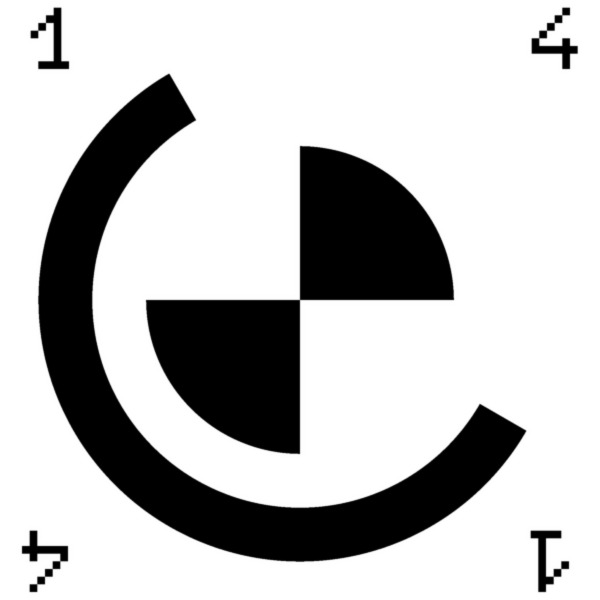
\includegraphics[width=4cm]{Methods/Images/IGN-14.jpg}
	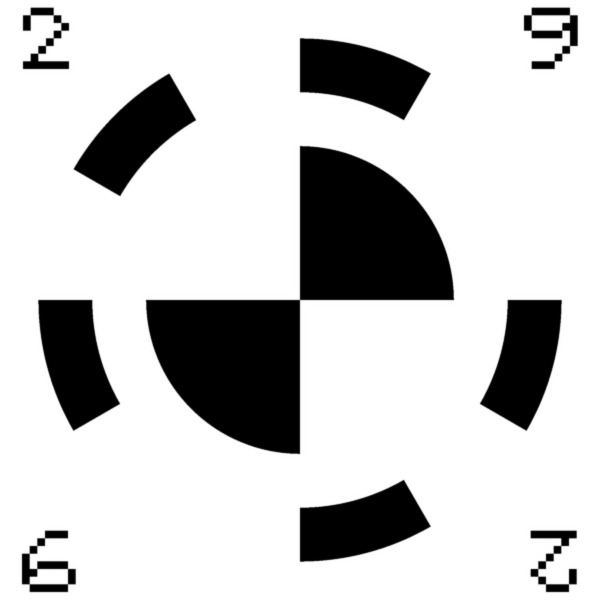
\includegraphics[width=4cm]{Methods/Images/IGN-29.jpg}
	\caption{Targets will long and short run for the same set}
\label{fig:CodeT:RL}
\end{figure}

Considering the robustness to false detections, we  use the following cautious criteria : "we want to be sure
that we will be able to detect an error as long as we have less that $N$  bits wrong detectected"
where $N$ is a given value.  It is easy to see that $N$  can be caraterized as the minimal hamming 
distance between all the selected pair of code.
The haming distance $D_H$ , being classically the number of bit different between two code, for example:

\begin{equation}
	D_H(10001,11001) = 1
\end{equation}

Also when we consider that codes are identic up to a certain subset $S$ of circular permutation,
we have to take care of that in definition of a haming-quotient distance $D^S_H$ :
 obvioulsy if $5 \sim 514 $ we must consider that $D^S_H(5,514)=0$,  or also $D^S_H(4,514)=1$ because
 $5 \sim 514 $ and $D_H(4,5)=1$ .  From a generam and formal viewpoint, we will write  :

\begin{equation}
	D^S_H(V_1,V_2) =  Min_{s\in S} D_H(V_1,s(V_2))
\end{equation}

%-----------------------------------------------------------------------
%-----------------------------------------------------------------------
%-----------------------------------------------------------------------

\section{Circular target detection}

In this section we make a brief description of the method used for 
detection of circular target detection implemented in {\tt MMVII}.
This descrition is made mainly to have a better understanding of the code and dont
make a complete justification of the approach.



The basic idea, is that localy the image deformation can be accurately approximated
by a affine function, then the target,  originally circular, is an ellipse in the image.
The main step of the pipeline are :

\begin{itemize}
       \item detection of the seed points, these point are the point at the top of target;

       \item estimation of radiometry : black and white of the target in image;

       \item computation of the connected component of the seed points, and of its frontier;

       \item estimation of an ellipse parameter and validation/invalidation;

       \item computation of the an image in polar coordinates to make the code linear.

\end{itemize}


%-----------------------------------------------------------------------
\subsection{Seed detection}

The seed detection is the very first part, at this step all the pixel are analysed,
so it must be very fast, must omit (almost) no pixel-seed for true ellipse; on the
other hand we accept a relatively high over detection as long as we are sufficiently
selective to allow more sophisticated filtering after 

Assuming that the shape is an ellipse (so a convex shape)
it has a single point that it maximal in one direction (whatever maybe be this direction).
We, arbitrarily select the up-vertical direction and try to detect these points using a
series of following criteria :

\begin{itemize}
      \item  it  is a point where gradient in $y$ is positive;
      \item  it  is point where gradient in $x$ change of sign;
      \item  among the points described above, it is a point where gradient in $y$ is maximal
	      in a given neighboorhod (fix at $15$ pixel for now => change as function of diam min);
      \item  the contrast complies with some threshold criteria (fixed to very low value).
\end{itemize}

After such filtering, typically $0.003\%$ of the points are selected (on our test images) which
allow to have more intensive computation.  Left image of figure~\ref{fig:CodeT:Seed}, illustrate
the kind of resut we get at this step.

\begin{figure}
\centering
	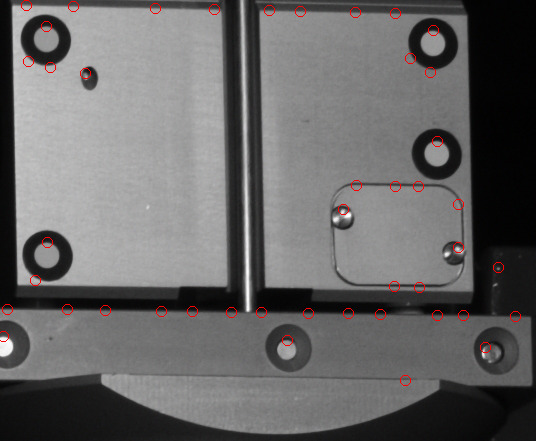
\includegraphics[width=6cm]{Methods/Images/Seed.jpg}
	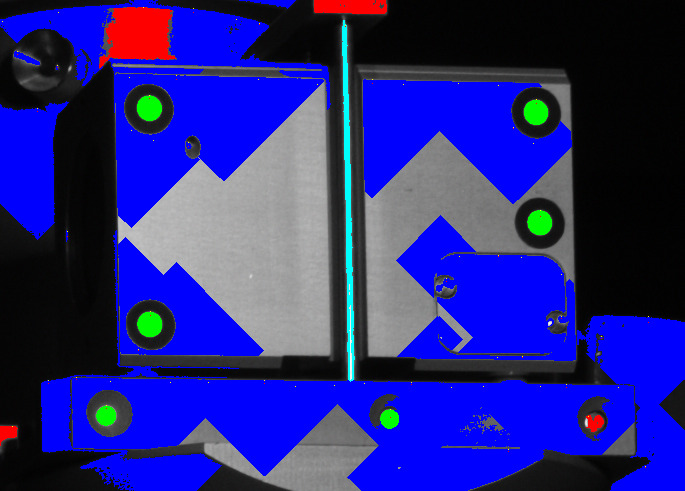
\includegraphics[width=6cm]{Methods/Images/ConnectedComp.jpg}
	\caption{Seed points and connected component}
\label{fig:CodeT:Seed}
\end{figure}

%-----------------------------------------------------------------------

\subsection{Radiometric modelisation and connected component analyisis}

In this document, we consider a white ellipse  on black background.  There is obvious
adaptation to do for black ellipse on white background.

The "real" target are black and white . We assume that locally, at the scale on one target in
one image, the image radiometry can be modelized as :  binary + some blurring + some  noise;
we also assume that locally the black and white of the target are maximal  (in a certain
neighbourhood there is no whiter than the white of the target ).
On the other hand, we consider that no  modelization of the radiometry can be made
at the level of a global image due to variation of lighting condition. Typically, 
the case we dont try to modelize is a target which woud be partially in the light and partially
in the shadow.

At this step, we must estimate the local value of black and white.  We search these
value on a vertical line crossing the seed point;  the function $Gray=F(y)$ is modelized
as a  Heavisied function (local binary) convoluted by  some gaussian blurr.
We start from the seed point, and use the following method :

\begin{itemize}
   \item  go up while gray level decrease, when reached this give the value of black $B$; 
   \item  go up down gray level increase, when reached  at a point $P_w$ this give the value of white $W$.
\end{itemize}

We define a first estimation of the ellipse as the connected component of point  such
that $I(x,y) >  \frac{B+W}{2}$ with $P_w$ as seed point of the connected component.
Right image of figure~\ref{fig:CodeT:Seed} present the kind of result we obtain at this step.

%-----------------------------------------------------------------------

\subsection{Ellipse estimation and validation}

Once we have the connected component, we extract the potential ellipse,
this done using the following process :

\begin{itemize}
	\item  extract the pixel (integer coordinate) that are the frontier of
		connected are;

	\item  refine their position to get real coordinate;  for this let $C$ be the
		centroid of connected zone (it will be approximatvely centrer of ellipse), let
		$P$ be a pixel frontier, we look for a point $Q$, after $P$
		on the direction $\overrightarrow{CP}$  such that $I(Q) = \frac{B+W}{2}$,
		using an interlpolation model for $I$ (the idea  is that, taking into account
		the blurring, the "real" ellipse is  $\pm$ the level
		curve of the gray corresponding to value between black and white);

	\item  estimate the ellipse parameter $ABCDEF$ by solving equation~\ref{ElEq}
		where $x,y$ are the coordinate of frontier points.
\end{itemize}

\begin{equation}
	A x^2 + B xy + C y^2 + Dx + E y = 1 \label{ElEq}
\end{equation}


We then tranformatet $ABCDE$ in "phypicall" parameter of ellipse : center, direction of great axe,
lenght of great an small axe  $C,\theta,L,l$.   The figure~\ref{fig:CodeT:Ellipse} presents
a global ellipse and a zoom on the frontier.

\begin{figure}
\centering
	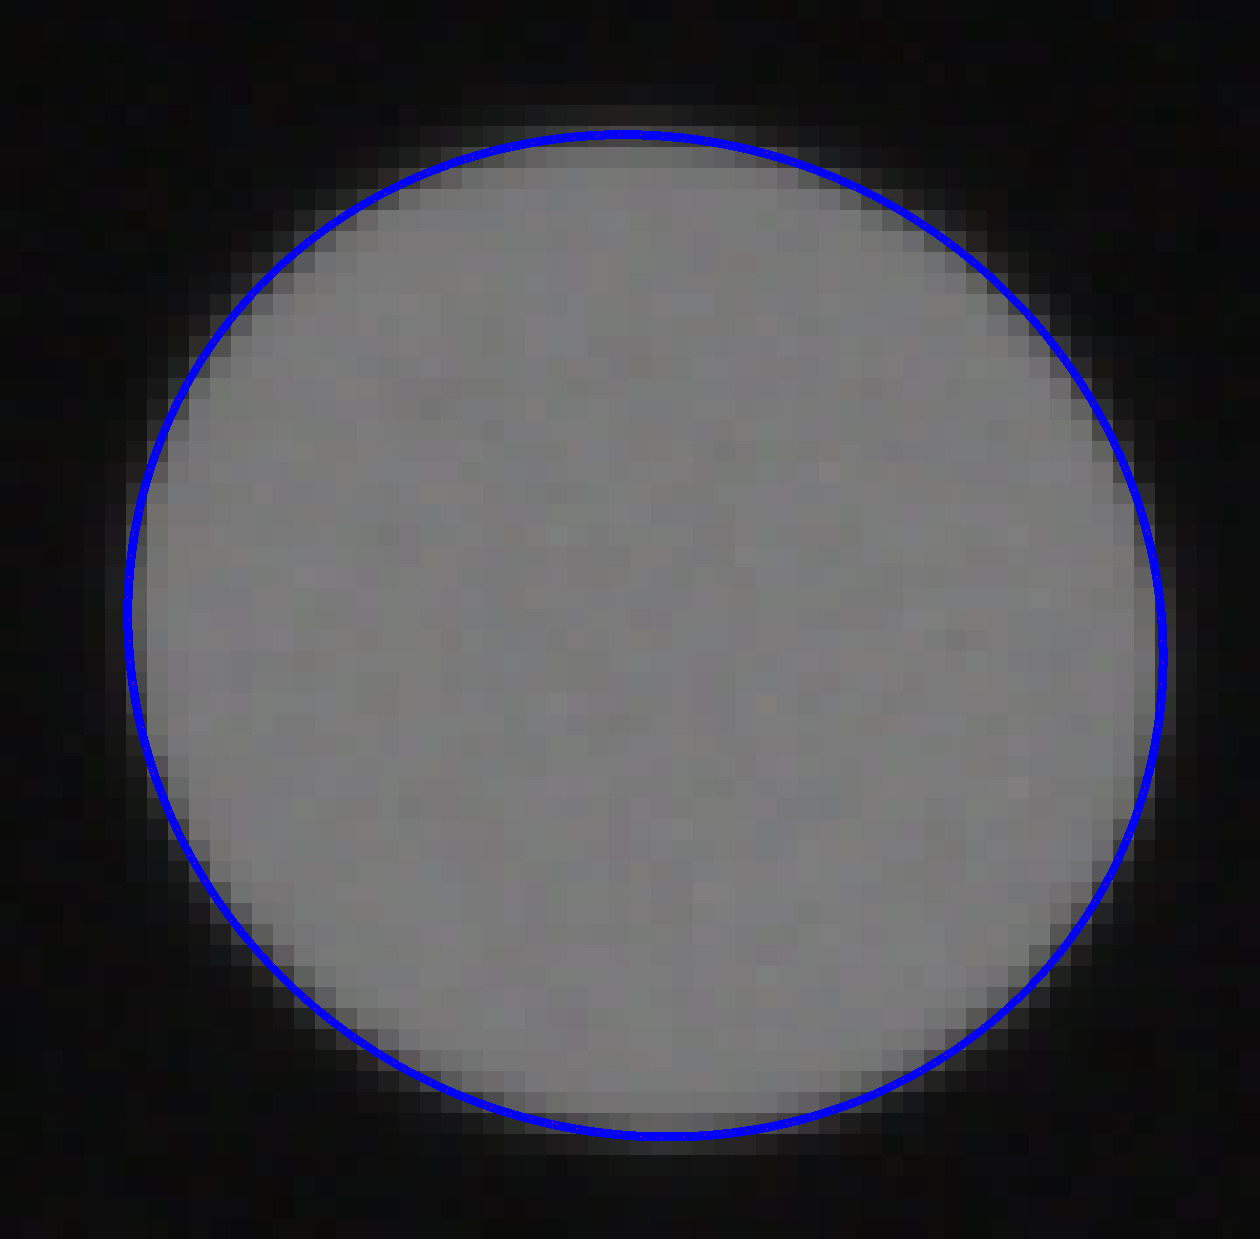
\includegraphics[width=6cm]{Methods/Images/FullEl.jpg}
	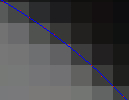
\includegraphics[width=6cm]{Methods/Images/ZoomEl.jpg}
	\caption{An extracted ellipse, and a zoom on the frontier : blue ellipse fitted on frontier points in red}
\label{fig:CodeT:Ellipse}
\end{figure}


Once the parameters are extracted, the ellipse is validated using two criteria :

\begin{itemize}
	\item  test on distance : average distance between frontier points and
		ellipse;

	\item  test on gradient : the ellipse is sampled, for each point theoreticall
		gradient is computed and compared to gradient extracted on image.
\end{itemize}

%-----------------------------------------------------------------------

\subsection{Code extraction and validation}

For this part, we consider that the coding system has a total circular permutation
amniguity as described in~\ref{GenEncodS} ($V \sim s(V)$ for any circular shift $s$).

\begin{figure}
\centering
	
\includegraphics[width=6cm]{Methods/Images/ZoomElCoded.jpg}
	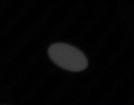
\includegraphics[width=6cm]{Methods/Images/ZoomElUnCoded.jpg}
	
\includegraphics[width=12cm]{Methods/Images/Polar2.jpg}
	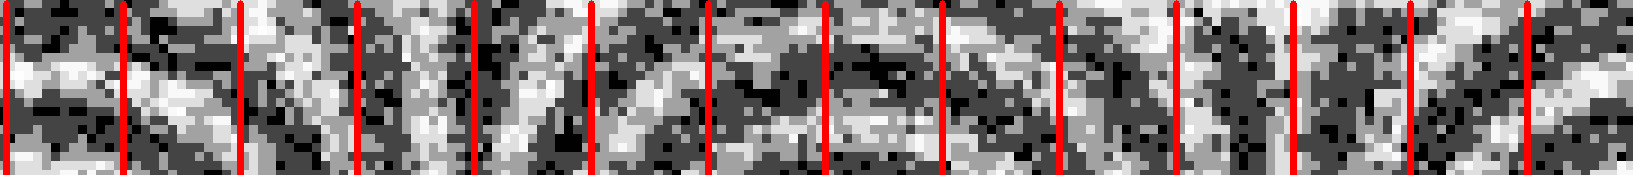
\includegraphics[width=12cm]{Methods/Images/Polar1.jpg}
	\caption{Extract of a coded an un-coded target, and the cooresponding polar image of their code
	(with dynamic enhancement), red lines are the computed offset}
\label{fig:CodeT:Ellipse}
\end{figure}


Once an ellipse has been validated and extracted , we must decide
if it is a coded target and, if it is, what is its code.  Let $C,\vec{u},\vec{v}$
be the repair of the ellipse, we will use the ellipse polar $\rho_i,\theta_i$
coordinates defined by :

\begin{equation}
	E(\rho_i,\theta_i) = C+L\vec{u}\rho_i \cos(\theta_i) +l\vec{v}\rho_i \sin(\theta_i) \label{Polar:Ellipse}
\end{equation}

Let $\rho_t,\theta_t$ be a polar coordinate system for the real tartget, such that  
the circle correspond to equation $\rho_t=1$. The transformation between the two system
is simply given by :

\begin{equation}
	\rho_i = \rho_t  \;\; ; \; \; \theta_i   =  \theta_t + \theta_0 \label{ElTargToIm}
\end{equation}

Where $\theta_0$ is certain offset that we cannot compute with only the ellipse extraction.
This is coherent : there is  $6$ unknown of affinity between image coordinates and taget coordinates,
and ellipse extraction has only given us $5$, so there remain at this step an unknown : $\theta_0$.

First we make a polar image using equation~\ref{Polar:Ellipse}.  
We cannot compute $\theta_0$ and we dont need it in fact, because the coding 
used is invariant to a circular shit. But we can an need to compute the phase $\phi_0$,
$\phi_0 \equiv \theta_0 \mod \frac{2 \pi}{N}$ where $N$ is the number of bit used for coding .
Let $\mathcal{I}^{k}_{\phi_0}$ be the interval corresponding to following definition :

\begin{equation}
	\mathcal{I}^{k}_{\phi_0} = [\phi_0 +\frac{2k \pi}{N},\phi_0 +\frac{2(k+1) \pi}{N}]
\end{equation}

Idealy, the polar image sould be constant on each interval $\mathcal{I}^{k}_{\phi_0}$, so 
to caracterize $\phi_0$ we compute it  as the value that minimize $\Sigma(\phi_0)$ 
the sum of standard deviation on each interval :

\begin{equation}
	\Sigma(\phi_0) =  \sum _k \sigma(\mathcal{I}^{k}_{\phi_0})
\end{equation}

The vertical red line of figure \ref{fig:CodeT:Ellipse} present the result of such computation.
Once we have compute $\phi_0$ we can compute for each interval $\mathcal{I}^{k}_{\phi_0}$ its 
bit-code by simply thresholding its value with $\frac{B+W}{2}$. We now have a complete model
of potential coded target, we can now validate it,  we use the following criteria :

\begin{itemize}
       \item first, obviously we check if the code is valid (check is there exist a shift $s$ such
	     that $s(V)$ is good code);

       \item then we check that radiometry is constant inside each $\mathcal{I}^{k}_{\phi_0}$
             by computing the ratio $\frac{\Sigma(\phi_0)}{\Sigma}$ where  $\Sigma$ is
             the standard deviation on the whole angles;

        \item  knowing the code, we can compute the theoreticall gradient at the limit of code :
               tangent transition between $0$ and $1$ , or radial transition between bit to foreground
               and background;

        \item \emph{we dont use} a criterion such that global homogeneity on the black (or white) part
              because, on the data set we use, there exist some linear bias due to lighting,
		as illustrated on figure~\ref{fig:CodeT:EllipseBias}
	
\end{itemize}


\begin{figure}
\centering
	
\includegraphics[width=5cm]{Methods/Images/Cro-Init.jpg}
	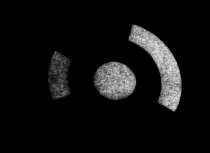
\includegraphics[width=5cm]{Methods/Images/Cro-EnhW.jpg}
	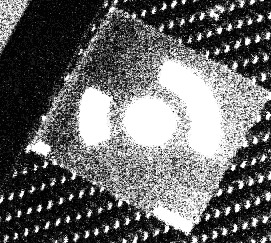
\includegraphics[width=5cm]{Methods/Images/Cro-EnhB.jpg}
	\caption{Target with lighting creating biais}
\label{fig:CodeT:EllipseBias}
\end{figure}


  %  -  -  -  -  -  -  -  -  -  -  -  -  -  -  -  -  -  -  -  -  -  -  -  -  -  -  -  -  -  -  -  -

%-----------------------------------------------------------------------
%-----------------------------------------------------------------------
%-----------------------------------------------------------------------

\section{Checkboard target detection}

This section mixes methologicall aspects and reference to the implementation 
(names {\tt files}, names of {\tt classes, methods} \dots).

     %-----------------------------------------------------------------------

\subsection{Global architecture}

The main steps of the methods are :

\begin{enumerate}
       \item find potential center of checkboard , this is done on neigboorhing small enough not
             to include the limit of ellipse ;

     \item estimate the direction of $2$ axes  (still on neigboorhing small enough) , by sweeping direction arround
	     the center;

     \item estimate the local value of black and white on small neighbourhood;

     \item estimate the black points of checkboard by a component analyis (of point under gray threshold) ;
           then estimate  point of ellipse frontier caracterised as frontier point of the connected component  that are not 
	   close to the axes;

     \item estimate the ellipse (with center fix) from the frontier point by least square, 
           then estimate the corner of the checkboard by intersection of the ellipse and the axes,
           then estimate the affinity between image and reference target;

      \item finaly decode \dots 
             
\end{enumerate}


     %-----------------------------------------------------------------------

\subsection{Find centers}

The computation of potential centers is made by application of successive criteria with
progressive elimination of candidate  by some thresholdings :


\begin{enumerate}
     \item  compute the points that are "tologically" saddle points (see~\ref{TopoSadlePoint});

     \item  refine the position of these points by fitting a quadratic function  on image,
	     and extract the null gradient point;
             compute the curvature;

     \item  use the curvature criteria to select a subset of point on global and local criteria;

     \item  compute a symetry criteria, use-it to refine the position and select point on a thresholds on
	    this criteria.
\end{enumerate}

Note the implementation use a series of classes included like \emph{matriochka} (russian dolls) ;


\begin{enumerate}

	\item the smallest \emph{doll} is class  {\tt cCdSadle} that represent candidate selected 
		at first level as saddle point criteria;

	\item the we have {\tt cCdSym} that represent a candidate selected on symetry criteria, 
              a {\tt cCdSym} is also a {\tt cCdSadle},
		and we have in the implementation
		"{\tt cCdSym}  \emph{inherits} of {\tt cCdSadle}"
		\footnote{what we write  {\tt cCdSadle} $\prec$ {\tt cCdSym} }

        \item the scheme is followed all allong the progression;

	\item globally we have    {\tt cCdSadle} $\prec$ {\tt cCdSym}  $\prec$ {\tt cCdRadiom} 
		$\prec$ {\tt cCdEllipse } $\prec$ {\tt cCdMerged } .



\end{enumerate}


  %  -  -  -  -  -  -  -  -  -  -  -  -  -  -  -  -  -  -  -  -  -  -  -  -  -  -  -  -  -  -  -  -
\subsubsection{tological saddle points}
\label{TopoSadlePoint}




